% =========================================================
% CONFIGURACION DEL DOCUMENTO
% =========================================================
\providecommand{\main}{..}
\documentclass[\main/main.tex]{subfiles}

% =========================================================
% CONTENIDO
% =========================================================
\begin{document}
\chapter{Resultados}
\label{cha:04_resultados} 
    % Debido a las características de este trabajo de título se opta por presentar los resultados obtenidos a modo de manual de uso. En este sentido, y dado que la aplicación puede ser utilizada tanto en forma de \textit{\acrshort{api}} como de \textit{GUI}, se decide presentar desde estas dos perspectivas el proceso de configuración y ejecución de un experimento.

    % El experimento a configurar estará conformado por dos tareas que se ejecutarán una sola vez, de forma secuencial y luego de presionar la tecla espacio. La primera tarea a configurar consistirá en un ejercicio de movimiento prosacádico bajo el paradigma de \textit{overlap}, lo que implica que el estímulo central se encontrará presente en todos los cuadros. De esta forma, se propone un cuadro inicial que contenga solo dicho estímulo identificado por una cruz blanca, con duración de $1.7[s]$. Luego, se presenta un cuadro que contenga además el punto objetivo identificado por un cuadro rojo, $16\degree$ a la derecha, durante $1.5[s]$. La segunda tarea consiste en la presentación de una imagen centrada para analizar patrones de búsqueda. En este caso el cuadro no debe ser temporizado: La tarea termina luego de que el usuario presione la tecla espacio. 

    % El perfil de configuración será configurado de forma tal de presentar los estímulos en el monitor secundario, ubicado a $53[cm]$ del usuario, con un ancho efectivo de $47.5[cm]$ y una resolución de $1680x1050[px]$. Además se hará uso de un \textit{eye tracker} ''Eyetribe'' y los resultados obtenidos serán almacenados en el directorio \textref{''C:/SaccadeApp/events/''}.

\begin{singlespace}\begin{python}
from saccadeapp.api import SaccadeDB

database = SaccadeDB(path=u"C:/SaccadeApp/")
\end{python}\end{singlespace}
        
\begin{singlespace}\begin{python}
from saccadeapp.api import Configuration

config_profile = Configuration(db=database)
config_profile.set_name(name=u"Test Profile (code)")
config_profile.set_events_path(path=u"C:/SaccadeApp/events/")
config_profile.set_tracker(tracker=u"eyetribe")
config_profile.set_monitor(monitor=u"My_Monitor")
config_profile.set_screen(screen=1)
config_profile.save()
\end{python}\end{singlespace}

\begin{singlespace}\begin{python}
from saccadeapp.api import Experiment, Test, Frame, Component

# Experiment:
experiment = Experiment(db=database)
experiment.set_code(code=u"exp_0001")
experiment.set_info(name=u"Example Experiment", version=u"coded_1.0")
experiment.set_descripton(text=u"This experiment was created with code!")
experiment.set_space_start(status=True)
experiment.set_dialog(status=False)
experiment.set_random(status=False)
experiment.set_rest_conf(status=False)

# Test: 
test = Test()
test.set_name(u"Example Test")

# Test - Frame_1: 
frame_1 = Frame()
frame_1.set_name(u"Test Start")
frame_1.set_color(u"black")
frame_1.set_as_task(False)
frame_1.set_time(1.0)
test.add_item(frame_1)

# Frame_1 - Component
fp = Component()
fp.set_name(u"FP")
fp.set_shape(u"cross")
fp.set_color(u"white")
fp.set_position(0.0, 0.0)
frame_1.add_item(fp)

# Test - Frame_2:
frame_2 = Frame()
frame_2.set_name(u"Test Image")
frame_2.set_color(u"black")
frame_2.set_as_task(True)
frame_2.set_keys_allowed(u"space")
frame_2.set_keys_correct(u"space")
test.add_item(frame_2)

# Frame_2 - Component
img = Component()
img.set_name(u"Couple Image")
img.set_position(0.0, 0.0)
img.set_image(u"couple.png")
frame_2.add_item(img)

experiment.add_item(test_1)
experiment.sequence_add(item_id=0, quantity=1)
experiment.save()
\end{python}\end{singlespace}

\begin{singlespace}\begin{python}
from saccadeapp.app import ExperimentHandler
handler = ExperimentHandler()
handler.prepare(exp_code=u"exp_0001", conf_name=u"Test Profile (code)")
handler.execute(frame_save=True)
\end{python}\end{singlespace}


\begin{figure}[H]
    \centering
    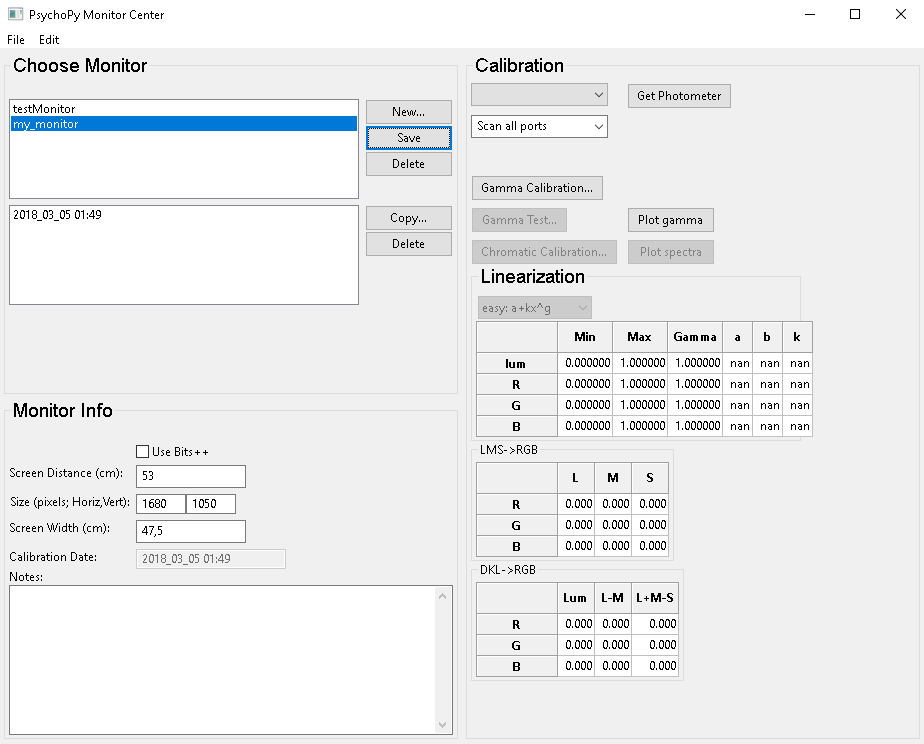
\includegraphics[width=0.6\textwidth]{cap_04_monitorcenter}
    \caption{Centro de monitores de PsychoPy.}
    \label{fig:04_monitor_center}
\end{figure} 


    \newpage
    \section{Comprobación de funcionamiento.}
    \label{sec:04_resultados}
        Para comprobar de que los datos estuvieran siendo registrados correctamente se creó un experimento cuya tarea principal solo contenía la imagen presentada en la figura \ref{fig:04_frame_result}.a. La tarea consistía en realizar una inspección visual, los resultados se presentan en \ref{fig:04_frame_result}.b.

        \begin{figure}[H]
            \centering
            \subfloat[Imagen original.]{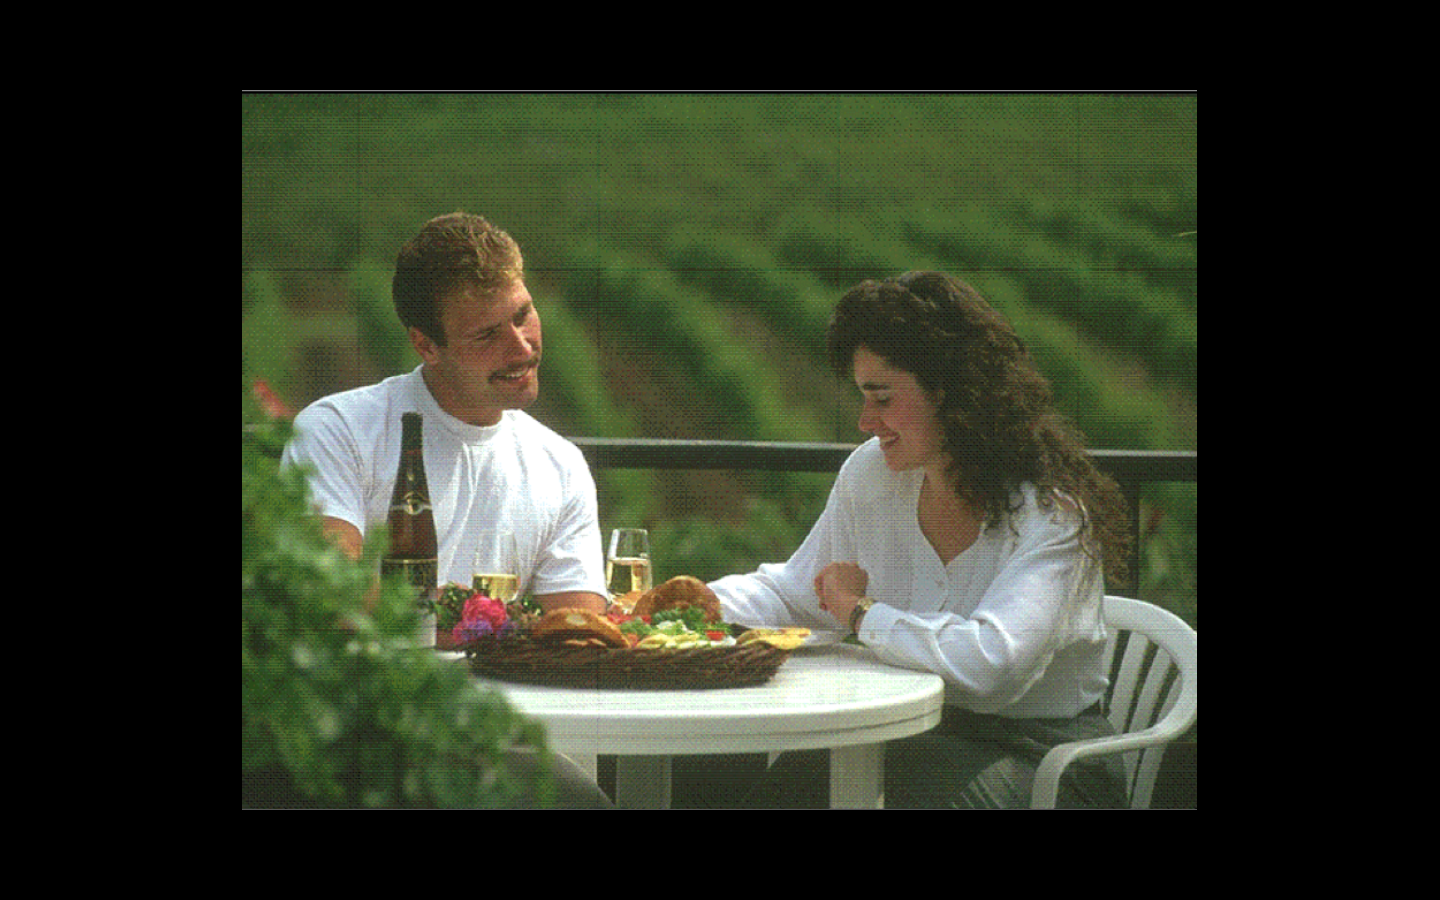
\includegraphics[width=0.45\textwidth]{cap_04_resultado_orig}}\\
            \subfloat[Movimiento ocular esperado.]{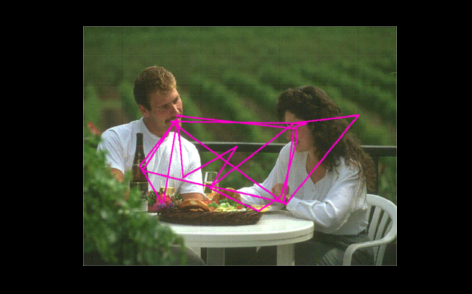
\includegraphics[width=0.45\textwidth]{cap_04_resultado_espe}}\hspace{5mm}
            \subfloat[Movimiento ocular registrado.]{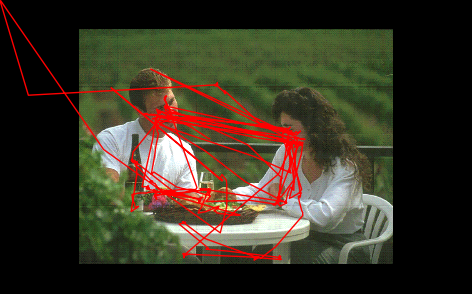
\includegraphics[width=0.45\textwidth]{cap_04_resultado_obte}}
            \caption{Datos registrados.}
            \label{fig:04_frame_result}
        \end{figure}

        Es posible apreciar en los datos registrados que el movimiento ocular en esta imagen se realiza principalmente entre los rostros de la pareja y las proyecciones de hacia donde se encuentran dirigidas sus miradas.

        Al consultar los registros de los puntos ubicados en la esquina superior izquierda y que parecieran no corresponder al patrón de observación se determina que estos corresponden a los momentos en que el usuario cierra los ojos.    

\end{document}
